\section{Analysis}

Building up on our initial idea and problem formulation, we determined two major functional areas that our must be supported by our proposed system:

\begin{itemize}[noitemsep]
    \item \textit{physical access control} (access to restricted premises in a company or institution, building access control etc.)
    \item \textit{online access control} (access to computer systems, applications, online sign-in etc.)
\end{itemize}

While the  typical question in a \acrshort{pacs}
% TODO check for usages in previous text. If it has not been used, then it should be \acrfull{}
would be ``\textit{Is the person allowed to enter beyond this point}?'', and can be controlled by a variety of physical barriers, doors, turn-sites and the like, the online access control is more complex. Enterprises nowadays operate a wide spectrum of software solutions including on-premise applications, legacy systems, cloud-based and \acrshort{saas} applications, internally or externally oriented \acrshort{api}s and databases. All of these require some level of access control. To break down this structure, we first begin by identifying two service classes:
\begin{enumerate*}[label=(\roman*)]
    \item \textit{internal applications}, that sit within the enterprise security realm; and 
    \item \textit{external applications}, that include cloud based software, \acrshort{saas} solutions and partner/vendor applications and which reside outside the given security realm.
\end{enumerate*}

The external applications can be further divided based on their interactions with said security realm. Applications that are not business critical and/or are not integrated with the business processes may not require access to protected resources at all. Examples of such applications would be a \textit{lunch booking system} or \textit{company social network}. These would be (primarily) used by the employees, but would not require connectors to business-critical system and could therefore reside outside the security realm.

Other external applications however, may require access to business-critical resources for their functions. \textit{\acrlong{crm}} or \textit{payroll} system may both be purchased as \acrshort{saas}, but both require connectors to protected resources to properly fulfil their functions. We can therefore extend our classification of external applications accordingly - applications that
\begin{enumerate*}[label=(\roman*)]
    \item \textit{require access to protected resources} and
    \item \textit{do not require access to protected resources}.
\end{enumerate*}

The access control of \textit{internal applications} will likely differ from access control of \textit{external applications} and similarly, access control will differ for applications that \textit{require} and \textit{do not require} access to protected resources. We can therefore devise an access control breakdown chart, as shown in Figure~\ref{fig:acs-classification}. Multiple sources list Identification, Authentication and Authorisation as crucial steps in access control. 
% REFERENCE 3x "CISSP Certification All-in-One Exam Guide" "Access Control Systems" "Identification, Authentication, and Authorization"
We focus on strong authentication and authorisation in the system design. 

\begin{figure}[ht]
    \centering
    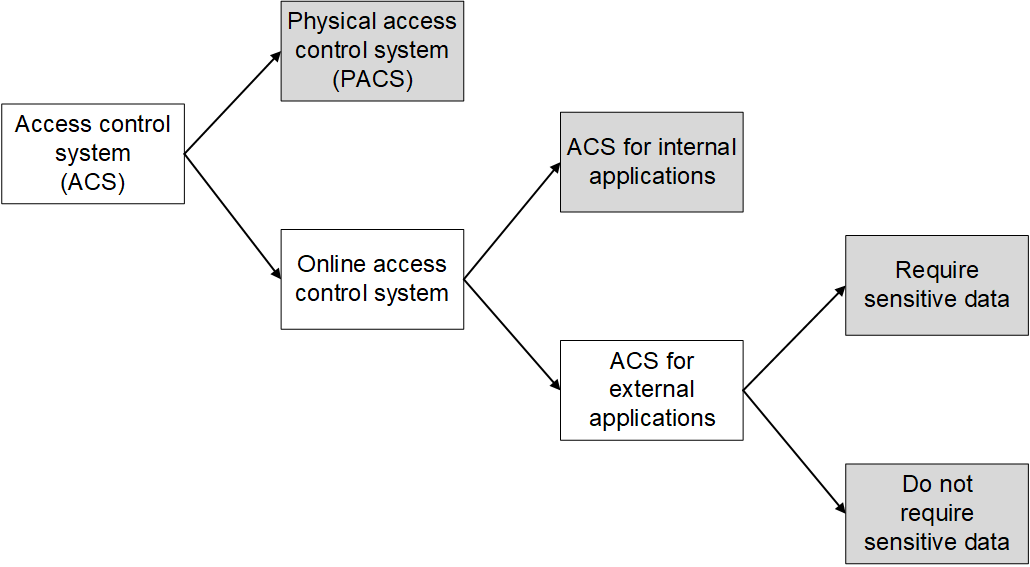
\includegraphics[width=.95\textwidth]{acs-classification}
    \caption{Access control system breakdown chart. \acrshort{acs} for external applications is different for applications work with sensitive data from \acrshort{acs} for external applications that do not work with sensitive data.}
    \label{fig:acs-classification}
\end{figure}

\paragraph{Authentication}
In \acrshort{pacs}, physical tokens, such as ID cards, are common practice nowadays. A survey carried out in 2016 indicated, that above 40\% of the companies rely on 125kHz proximity card, which are not considered secure. On the other end of the spectrum, around 20\% of the companies indicated use of mobile devices as a part of their \acrshort{pacs} solution. 
% REFERENCE "THE STATE OF PHYSICAL ACCESS CONTROL: IMPACT ON THE ENTERPRISE"
The main benefit of using mobile device for this purpose is, that most people already own a smartphone and usually carry it with them at all times. Other technologies represented in the survey that are considered secure today, include iCLASS (contact-less card) and MIFARE DesFire (contact-less card). FIDO nor FIDO2 keys (NFC, Bluetooth, or other) are not mentioned in the survey, although compatible \acrshort{pacs} systems exist on the market today\footnotemark.
% 
\footnotetext{\url{https://web.archive.org/web/20190319221618/https://www.yubico.com/works-with-yubikey/catalog/modis/}, accessed 19 March 2019}

% For \acrlong{aal}s 2 and 3 defined in 
% %  REFERENCE SECURITY REQUIREMENTS FOR CRYPTOGRAPHIC MODULES
% , authentication must be carried out using at least two independent factors. This requirement, together with abandonment of memorised secrets results in adoption of new authenticators. These  authenticators should offer at better security as memorised secrets, while maintaining the same level of accessibility. In 


\subsection{Functional requirements}

